\begin{figure}[t]
\centering
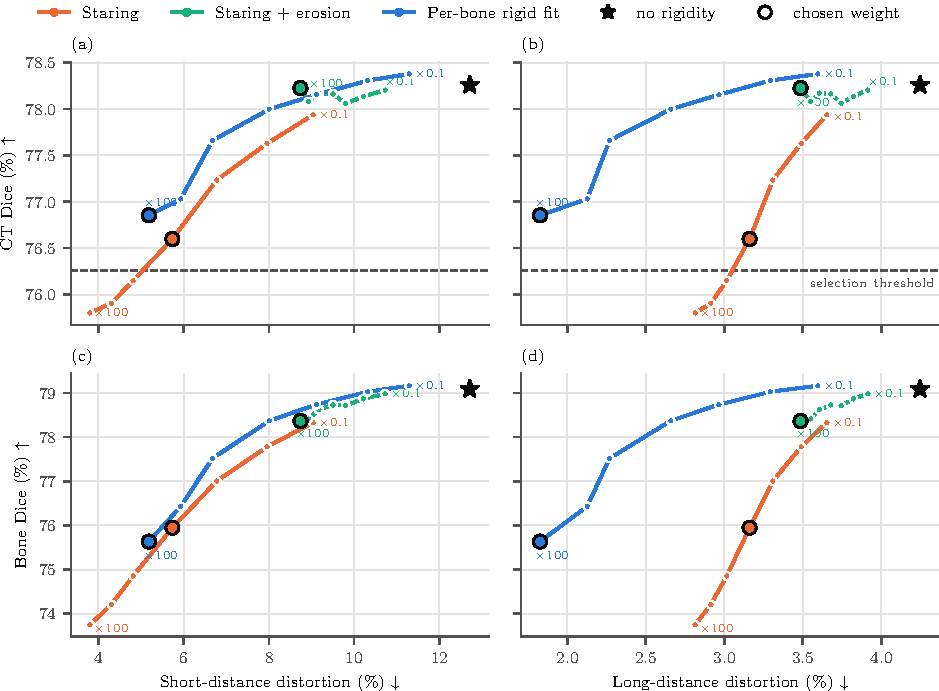
\includegraphics[width=\textwidth]{figures/rigidity.pdf}
\caption{Sweep of bone-rigidity weights on the validation set (26 patients, 38 pairs): network trained with the PET-preservation losses, followed by instance optimization (IO) with the PET-preservation terms and one bone-rigidity penalty at $0.1$ to $100$ times its calibrated reference weight (factors at the ends of each line).
Top: CT Dice; bottom: bone Dice; left: distortion of short (5--15~mm) and right: long ($\geq15$~mm) within-bone distances, defined as the mean absolute relative change in distance between point pairs in the same bone.
Color identifies the bone-rigidity penalty.
Star: IO without bone rigidity; dashed line in (a,~b): selection threshold two Dice points below the reference; outlined marker: weight chosen for the test set, the largest within the threshold up to $\times100$.
Points are means over patients after averaging each patient's pairs.}
\label{fig:rigidity}
\end{figure}
